\documentclass[11pt]{article}
\usepackage[utf8x]{inputenc}
\usepackage{fullpage}
\usepackage{enumerate}
\usepackage{gensymb}
\usepackage{mathtools}
\usepackage{standalone}
\usepackage{rotating}
\usepackage{lscape}
\usepackage{graphicx}
\usepackage{color}
\usepackage{listings}
\usepackage[framed]{mcode}
\usepackage{fullpage}
\usepackage[colorlinks=true]{hyperref}

\definecolor{lightgray}{gray}{0.5}
\setlength{\parindent}{0pt}

%opening
\title{CIS520 Final Project}
\author{Conor O'Brien \and Nick Iodice \and Siyao Hu}
\date{12/11/2014}

\begin{document}

\maketitle

\section{Results}

\subsection*{Methods}
\begin{enumerate}
	\item \textbf{Ridge regression / DT bagged ensemble by city:} for each city, trained ridge regression and TreeBagger ensemble (35 trees) on the residual
	\item \textbf{Ridge regression by city:} for each city, trained ridge regression
	\item \textbf{K-Means:} Used semi-supervised K-Means to cluster the data into three clusters, and trained a ridge regression model on each cluster. 
	\item \textbf{PCA w/ Ridge regression by city:} Used the top 50 PCA components, calculated with the entire dataset of words and bigrams, and trained different  ridge regression models for each city.
	\item \textbf{PCA w/ Ridge regression by city, words only:} Trained ridge regression models for each city using the top 50 PCA components of just the word data.
	\item \textbf{Binning with base prediction:} For each city, trained ridge regression, which was split into 3 bins based on price predicted. The residual for each bin was then predicted using a TreeBagger ensemble (35 trees)
	\item \textbf{SVR by city:} For each city, trained Support Vector Regression using words+bigrams.
	\item \textbf{SVR by city, words only:} For each city, trained Support Vector Regression using only words.
\end{enumerate}

\subsection*{Results}
\begin{center}
\begin{tabular}{| l || r |}
\hline
\textbf{Methods}									&	\textbf{RMSE}   \\ \hline \hline
Ridge regression / DT bagged ensemble by city:  	&	0.6781 \\ \hline
Ridge regression by city:							&	0.7316 \\ \hline
K-Means: 											&	0.8084 \\ \hline
PCA w/ Ridge regression by city: 					&	0.8346 \\ \hline
PCA w/ Ridge regression by city, words only: 		&	0.8352 \\ \hline
SVR by city: 										&	3.4867 \\ \hline
SVR by city, words only: 							&	3.1001 \\ \hline
Binning with base prediction, 35 trees: 			&	0.6960 \\ \hline
\end{tabular}
\end{center}
\section{Analysis}

\subsection{Testing random models}
During an initial exploratory period, our time was spent testing a variety of models without thinking much about why we were choosing them. Of course, this left much to be desired. For example, running SVR gave us an RMSE of over 3, whereas K-Means (K = 3) gave us an RMSE around 0.80. We decided that we needed to be more deliberate in our choice of model, so we looked at the data using dimensionality reduction methods to see its natural clusters. This helped us learn that each city has a different distribution of words, and was critical in our decision to run separate models for each city. Doing this resulted in the largest increase in accuracy we obtained over the course of the project.

\subsection{Predict residual}
We found that when we used only a single model for prediction, the best RMSE we obtained was approximately 0.73. We think that the ridge regression wasn't able to capture the full complexity of the word structure. In order to remedy this, we decided to use the latent signal contained in the residual. The best results we got were by using ridge regression to predict a base price, followed by a regression decision tree ensemble to predict the residual. By using the decision tree, we were better able to capture the nonlinearities in the data set. Furthermore, splitting out the regression and decision trees on a per city basis allowed for even higher precision.

\subsection{Binning}
By binning the data according to actual prices and then training a ridge regression on each bin, the overall performance is much better than training ridge regression for each city according to cross validation. Thus a method that could accurately predict which bin a certain observation belongs to was necessary. Accordingly we tried SVM, NB, DT and LR, but none of these worked very well. The reason was likely that the data does not follow the assumptions of those models. Since ridge regression for each city worked fairly well, we had the idea to do binning according to predicted prices from this method, but never tried it. After the project review, we implemented a method that first gets base prediction using ridge regression for each city, and uses the predicted prices to allocate observations into three bins: below 8, between 8 and 14, and above 14. Then we used TreeBagger to predict the residual. The performance is better than many of our other methods, but still worse than our final submission.

\subsection{Cross validation on \# PCA loadings}
Using PCA will reduce the size of our model, and takes less time to predict. So we tried to get the best number of loading by cross validation in ridge regression. However, the cross validation error kept decreasing until 2000 loadings. Furthermore, using 2000 loadings gives poorer results than using the original data, and the model is actually larger and prediction slower because the data is no longer sparse. One major issue with our method was that we used both the words and bigrams, while actually the bigrams may not help.

\subsection{Testing on BIGLAB for speed}
After validating our model and submitting to the leaderboard, we found that our code, while only taking a few minutes to predict all 20307 prices on our laptops, took well over ten minutes on BigLab. We experimented with a few methods to speed up our predictions, but a general optimization using the MATLAB profiler worked well.
\subsubsection*{Original Code:}
\begin{lstlisting}
city = find(X_test(1:7));

base_fit = cvglmnetPredict(model.cvglmnet_fit{city}, X_test(8:end));
residual_fit = predict(model.tree_fit{city}, full(X_test(8:end)));

prediction = base_fit - residual_fit;
\end{lstlisting}

\subsubsection*{Final Code:}
\begin{lstlisting}
prediction = cvglmnetPredict(model.cvglmnet_fit{(X_test(1:7)==1)}, X_test(8:end)) - ...
	predict(model.tree_fit{(X_test(1:7)==1)}, full(X_test(8:end)));
\end{lstlisting}

By reducing the number of operations, and replacing the find with an logical indexing operation, we were able to rapidly increase the speed of our code. We also experimented with running our ridge regression using single precision variables rather than doubles, which was faster but didn't make enough of a difference. Most of our time was spent in the TreeBagger prediction, and as the cross validation accuracy tended to increase up to 75 trees, we ran the maximum we could while remaining under the time limit, which was 35 trees.

\subsection{Reducing Model Size}
Our first saved models were well above the 50MB limit, but we were able to shrink them after trying a few different methods. Initially we thought to try using a compression program, and use system calls to decompress everything during \texttt{init\_model}, but MATLAB already does a good job with compression while saving, and we were unable to get any size reduction. Eventually we switched the cvglmnet model to use single-precision floats rather than double-precision, and were able to strip out much unneeded information from our tree model by turning the TreeBagger object into a CompactTreeBagger object, which omitted everything from the TreeBagger model except the actual trees used for prediction. 

\section{Visualization}
Figure \ref{WordCloud} is a word cloud showing the most frequent words in the decision trees of the ensemble method mentioned in the first section, with larger font size reflecting higher frequencies. Figure \ref{LSI} shows the distribution of words in the decision tree, broken down by city. The words that best predict the residual from ridge regression are different for each city.

\begin{figure}
	\centering
	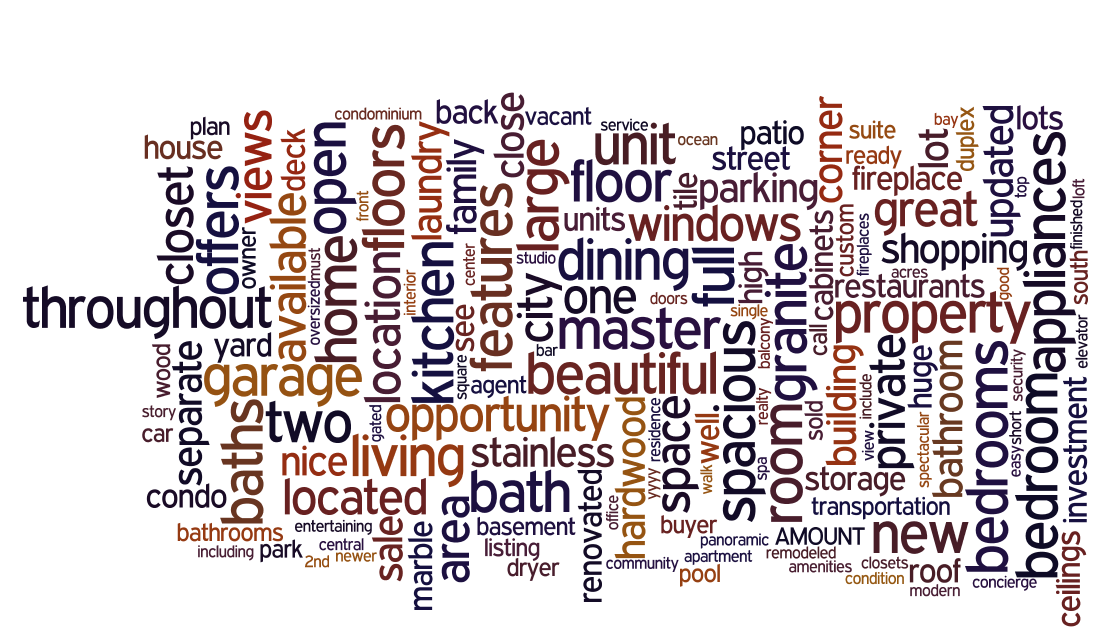
\includegraphics[scale=0.55]{word_cloud.png}
	\caption{Word Cloud from Frequency of Words in Decision Trees}
	\label{WordCloud}
\end{figure}

\begin{figure}
	\centering
	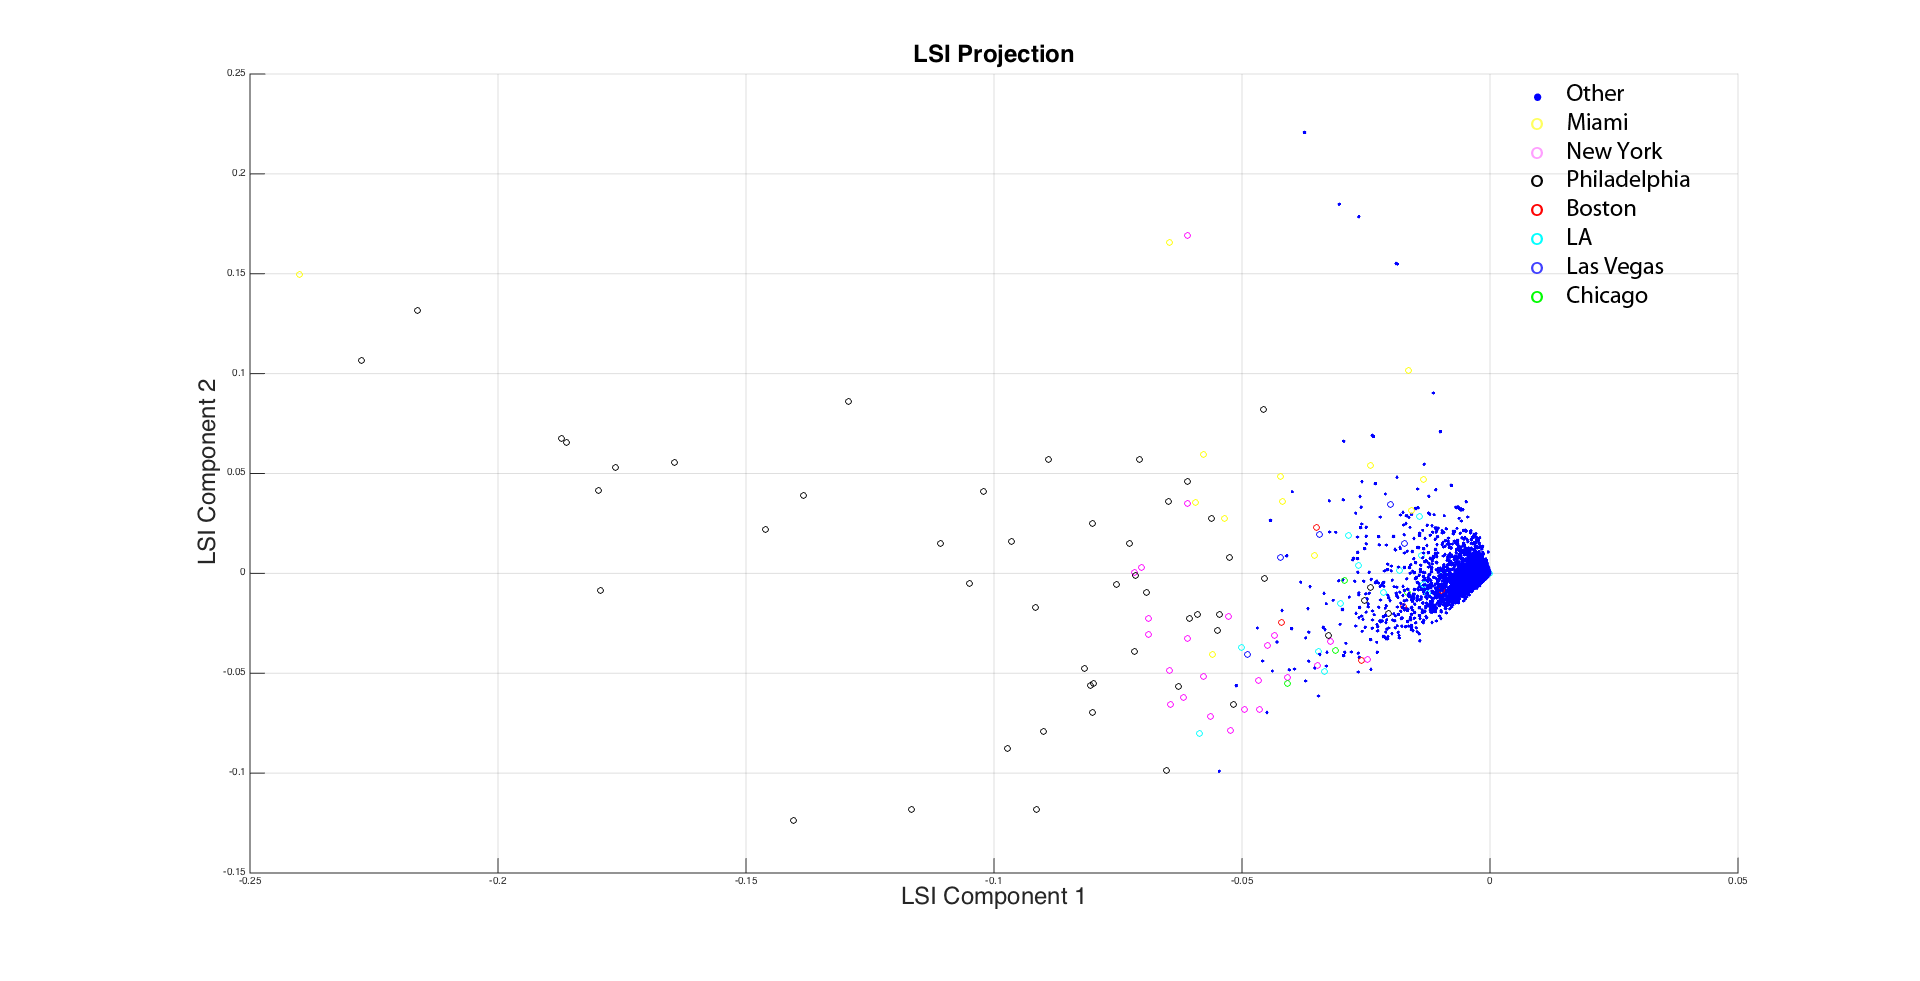
\includegraphics[scale = 0.30]{LSI_projection.png}
	\caption{LSI Reduction of Words Used by Decision Trees}
	\label{LSI}
\end{figure}

\end{document}